\chapter*{Motivation: Why Robots Need Math}
\markboth{Motivation}{Motivation}
\addcontentsline{toc}{chapter}{Motivation: Why Robots Need Math}

\section*{A flip that looks easy}
Look at the pictures below. A humanoid robot, the Booster K1, jumps, rotates backwards through the air and lands on its feet again: a \emph{webster flip}. A human gymnast needs years of training for a move like this. A robot has to do it with motors, sensors and a program, and every single frame of the motion is decided by mathematics.

\begin{figure}[htbp]
	\centering
	\begin{subfigure}[b]{0.19\textwidth}
		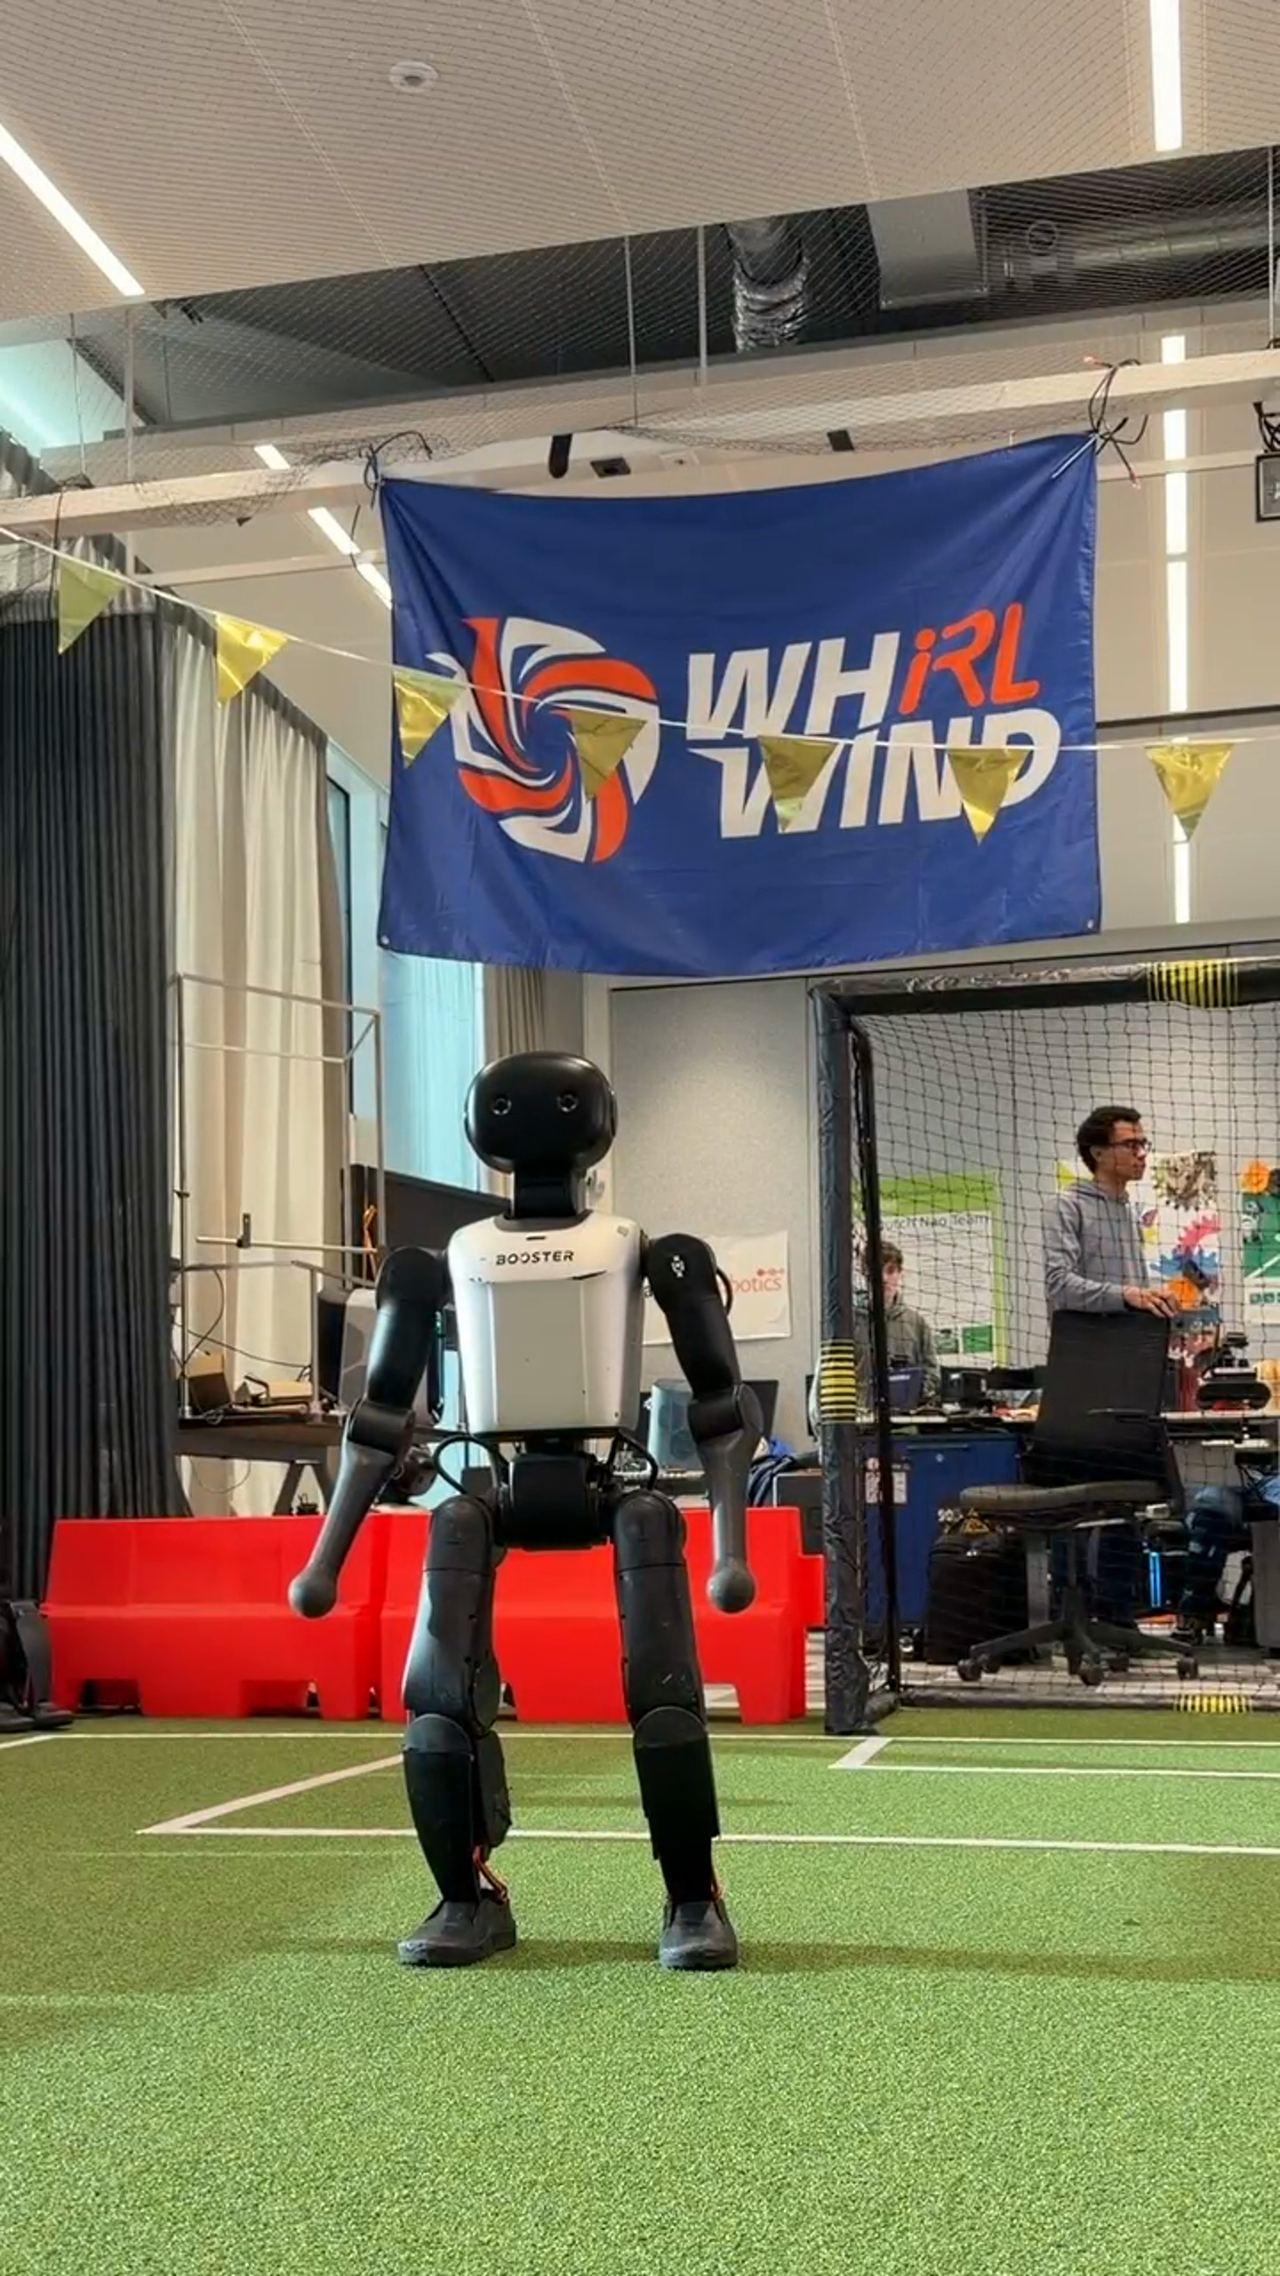
\includegraphics[width=\linewidth]{webster_flip/01.png}
	\end{subfigure}\hfill
	\begin{subfigure}[b]{0.19\textwidth}
		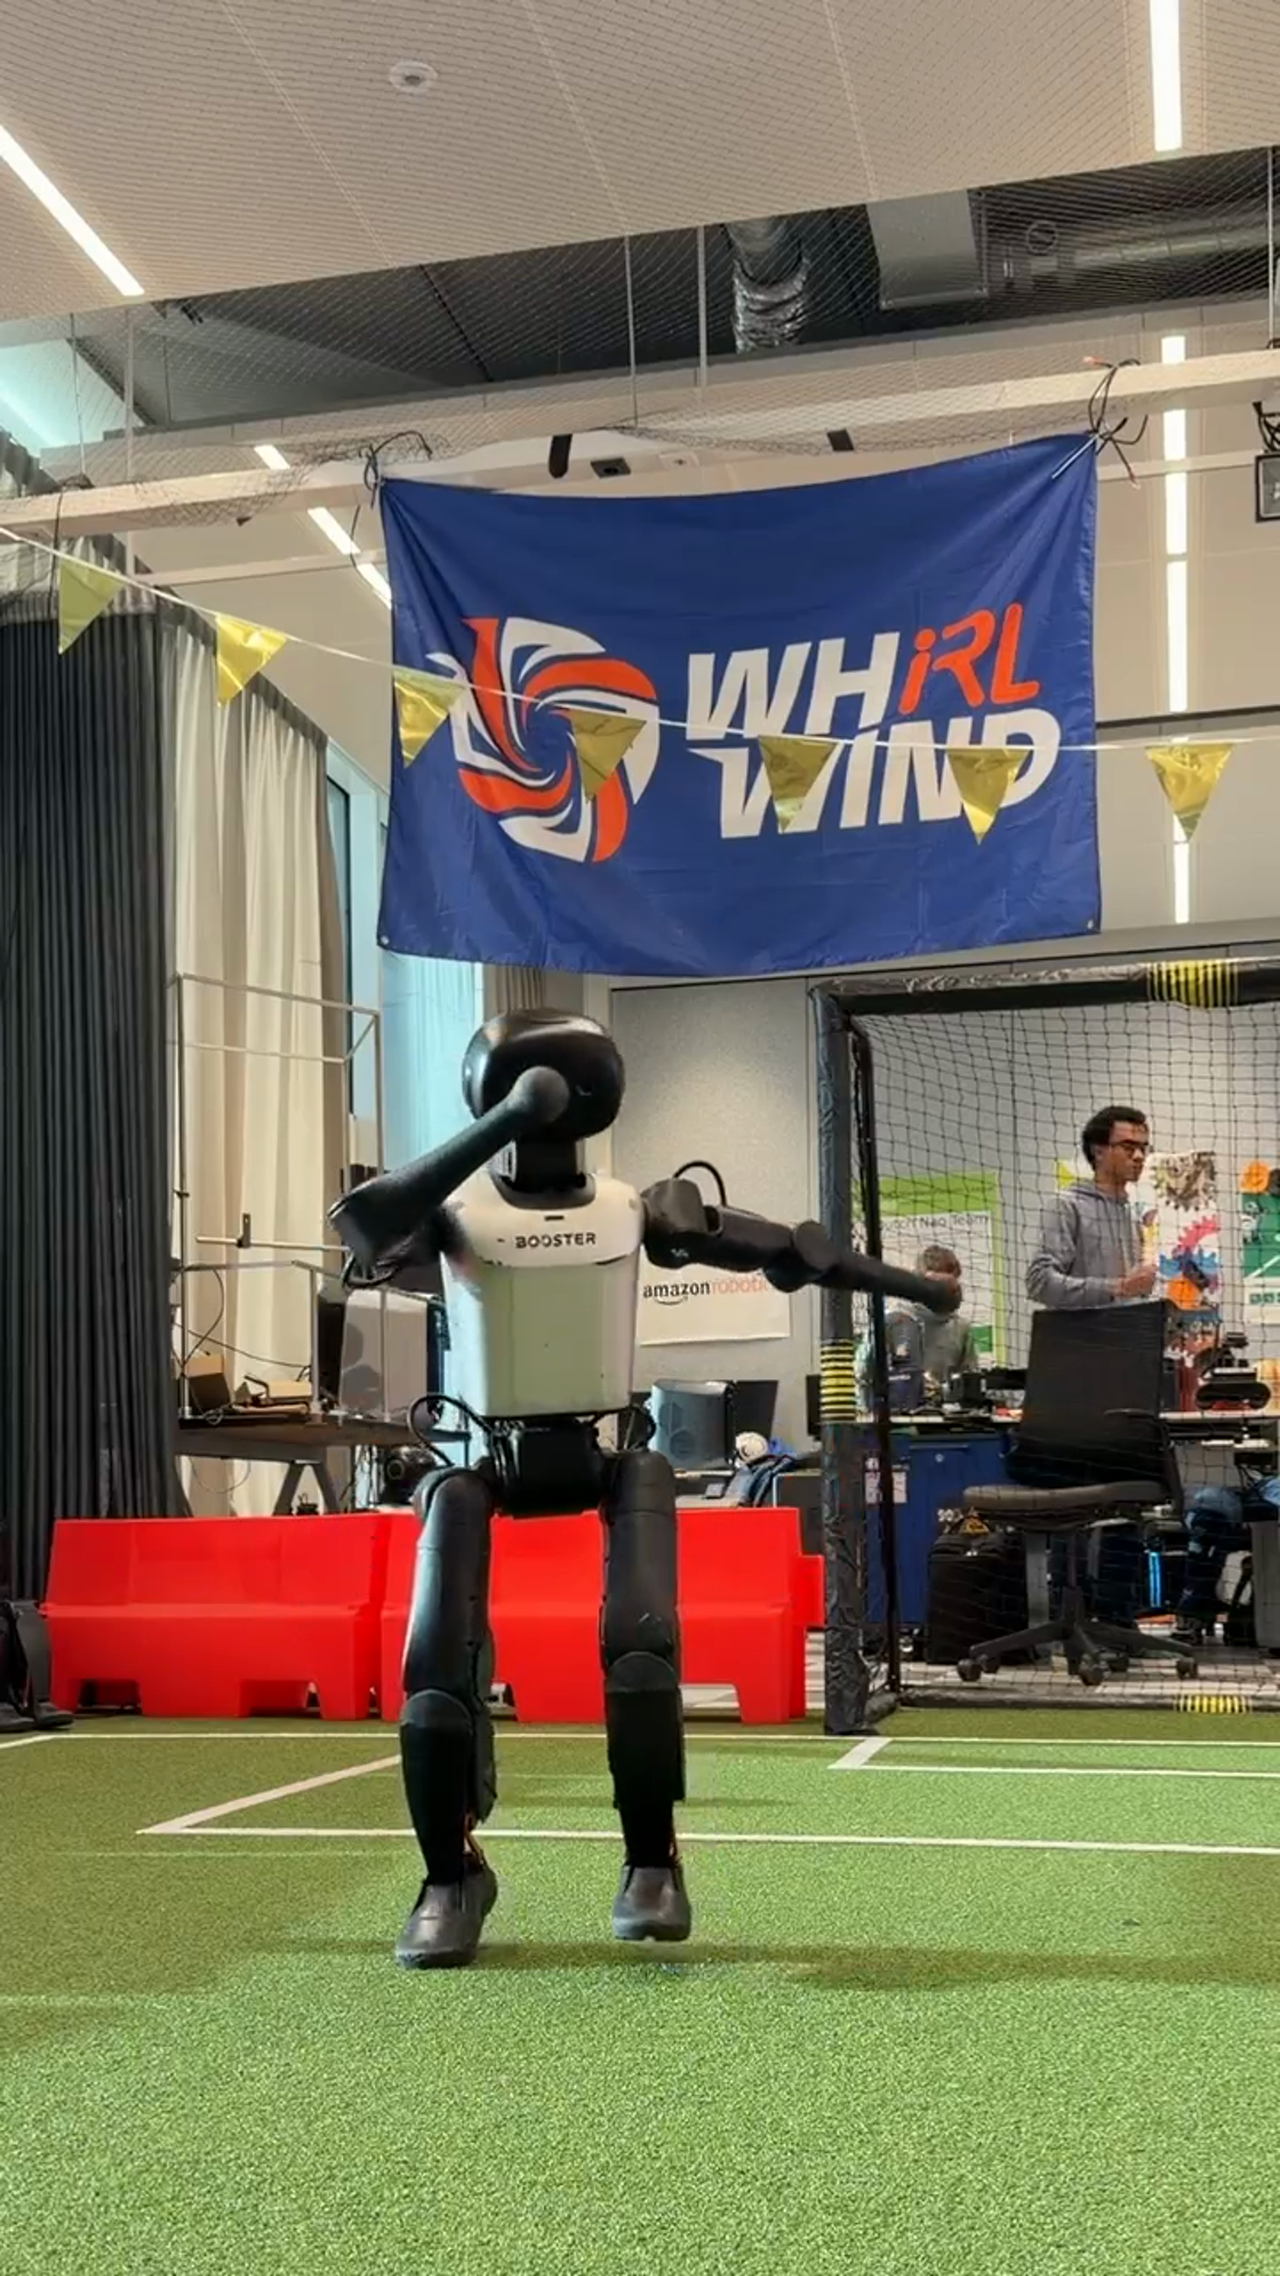
\includegraphics[width=\linewidth]{webster_flip/02.png}
	\end{subfigure}\hfill
	\begin{subfigure}[b]{0.19\textwidth}
		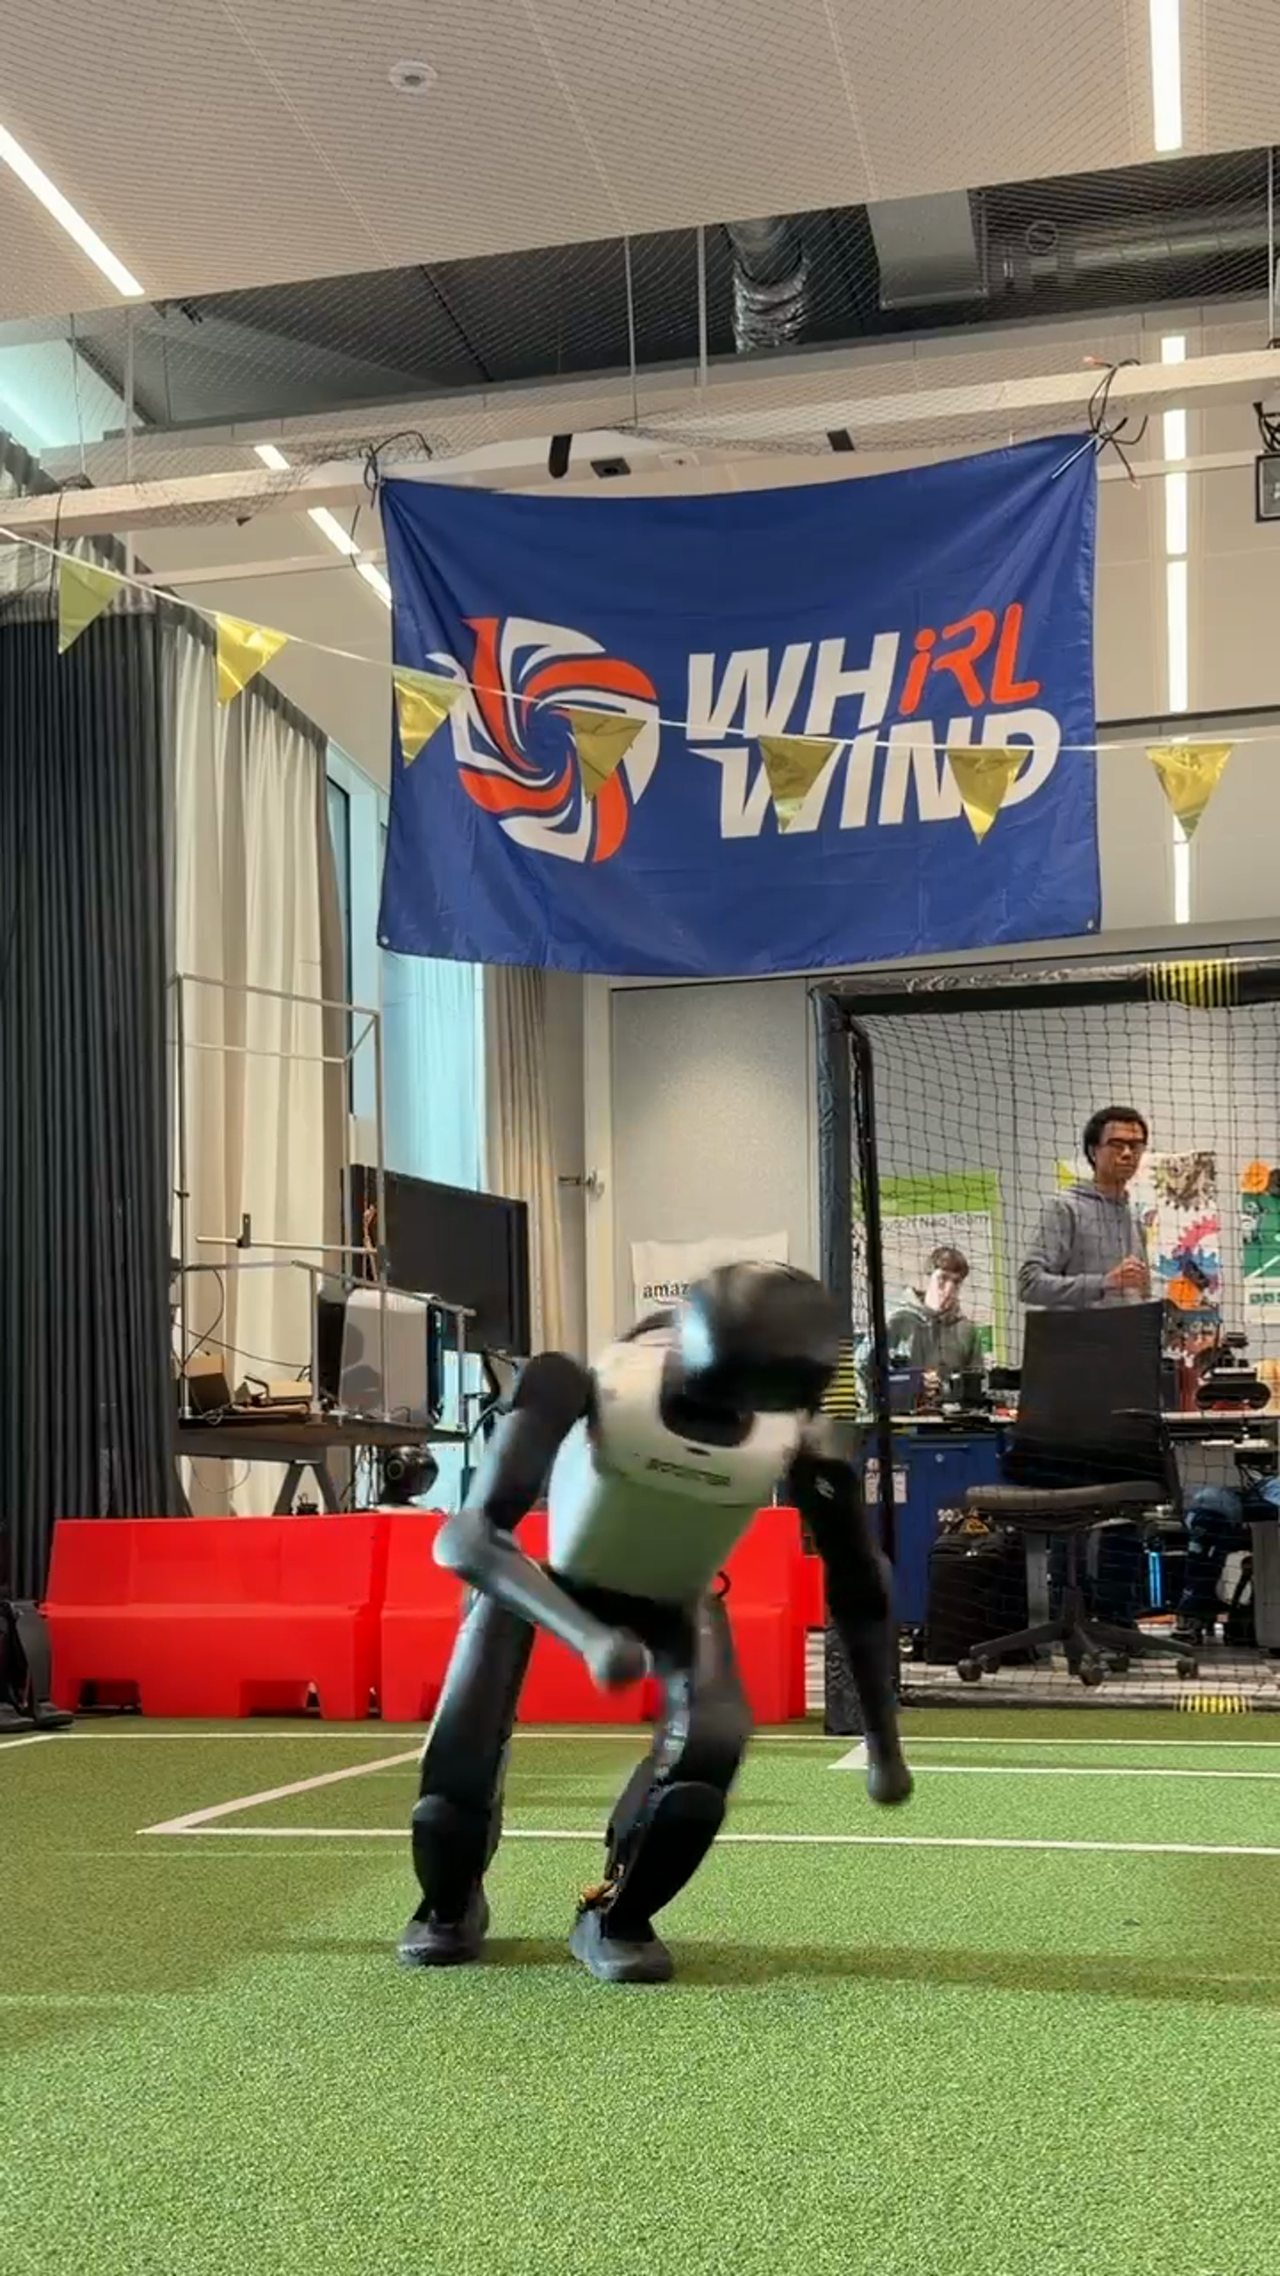
\includegraphics[width=\linewidth]{webster_flip/03.png}
	\end{subfigure}\hfill
	\begin{subfigure}[b]{0.19\textwidth}
		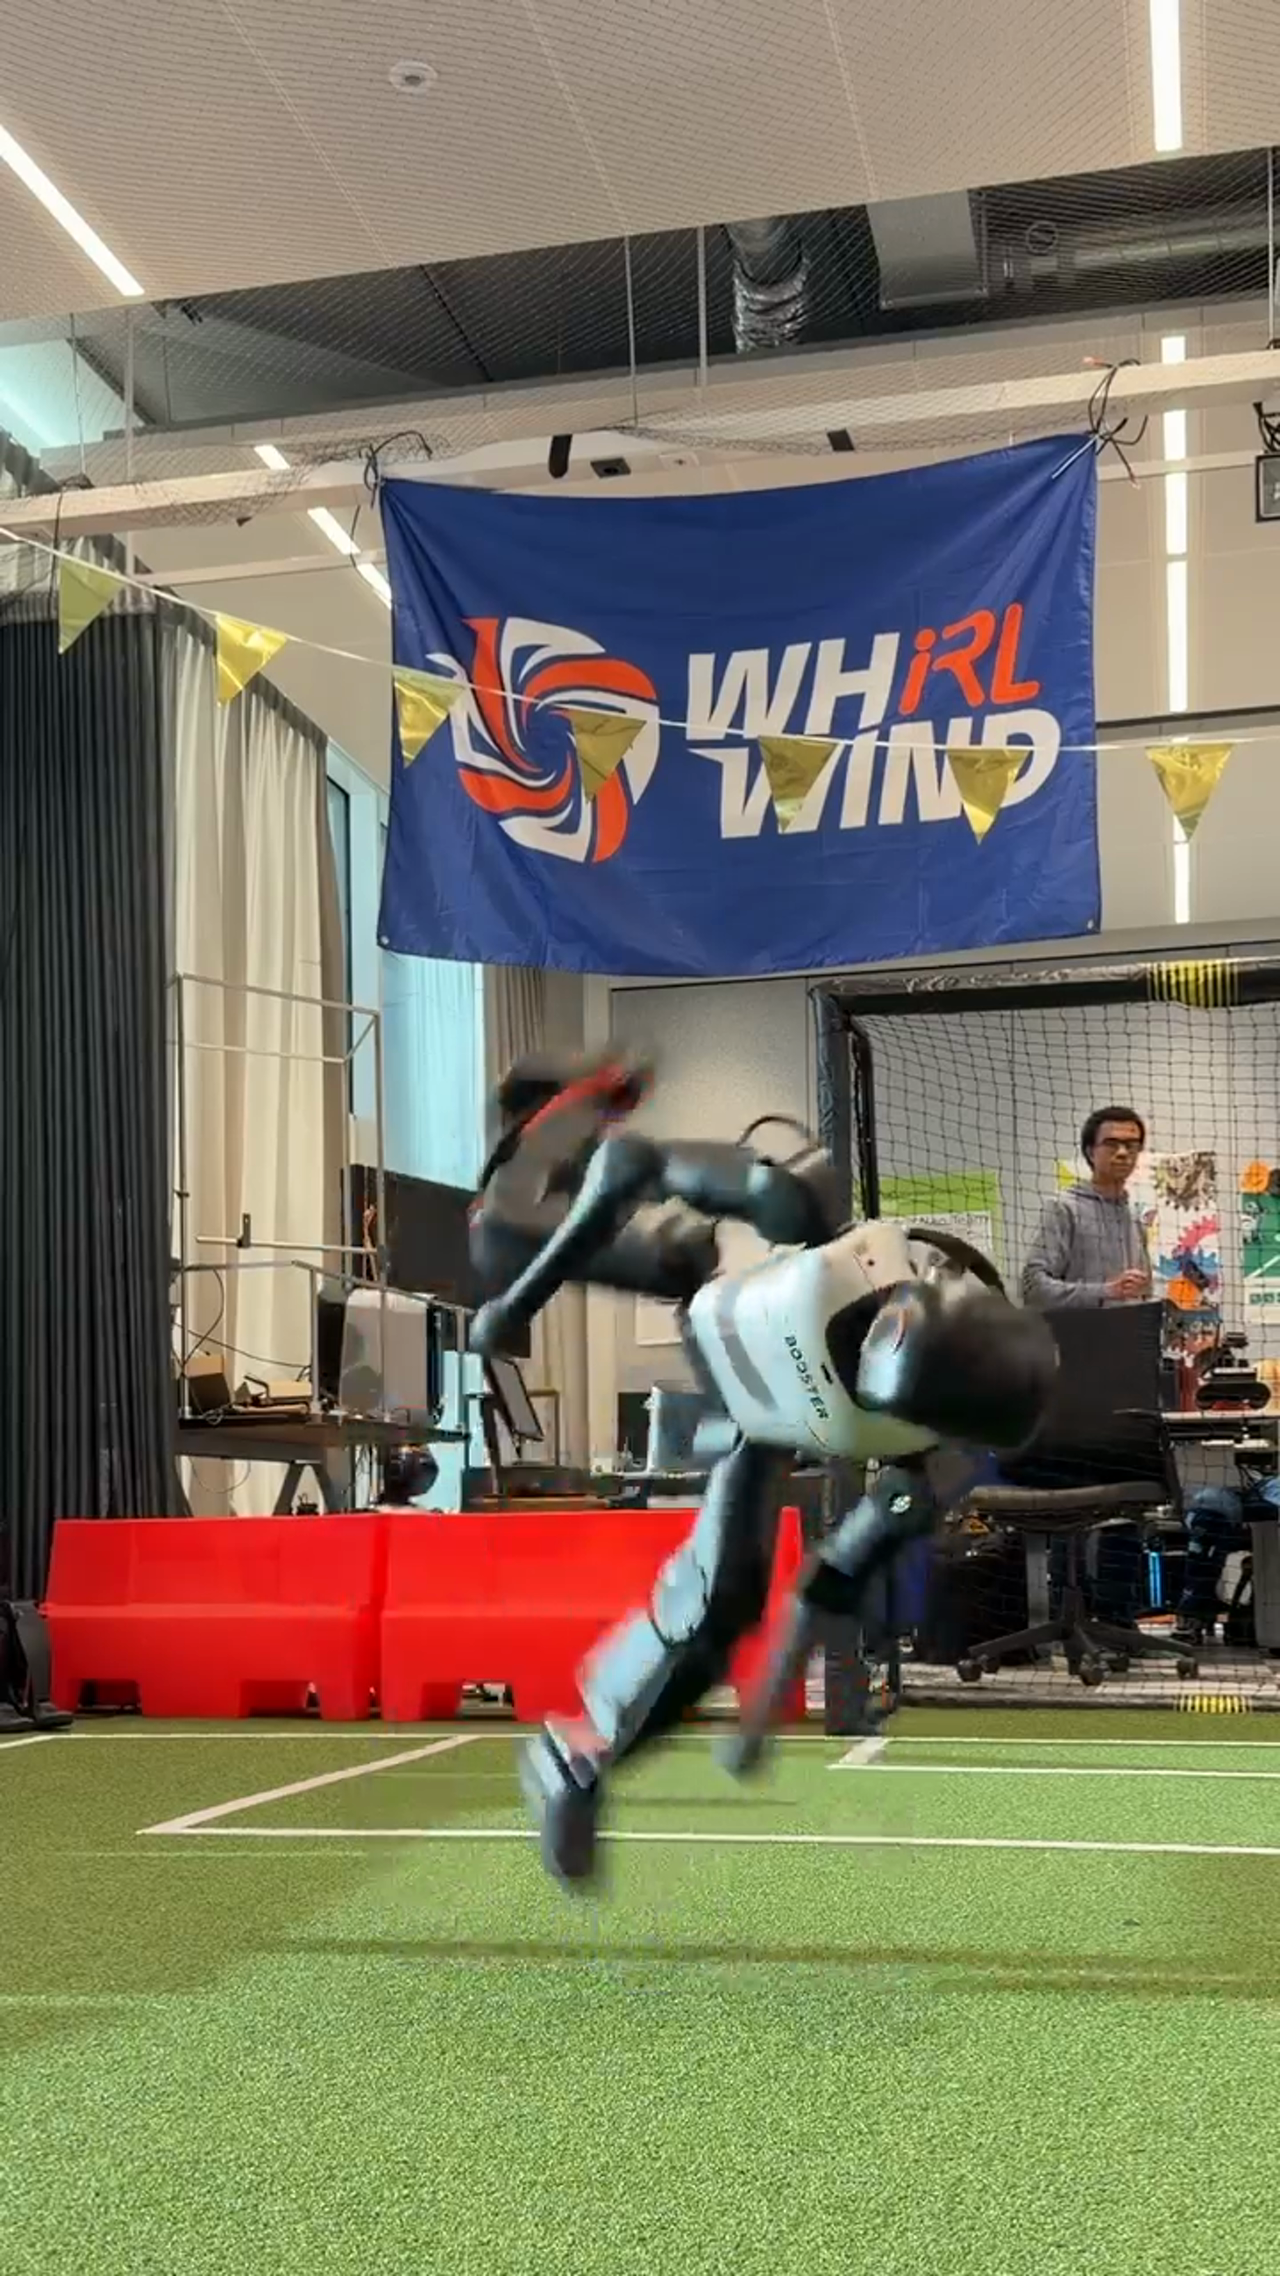
\includegraphics[width=\linewidth]{webster_flip/04.png}
	\end{subfigure}\hfill
	\begin{subfigure}[b]{0.19\textwidth}
		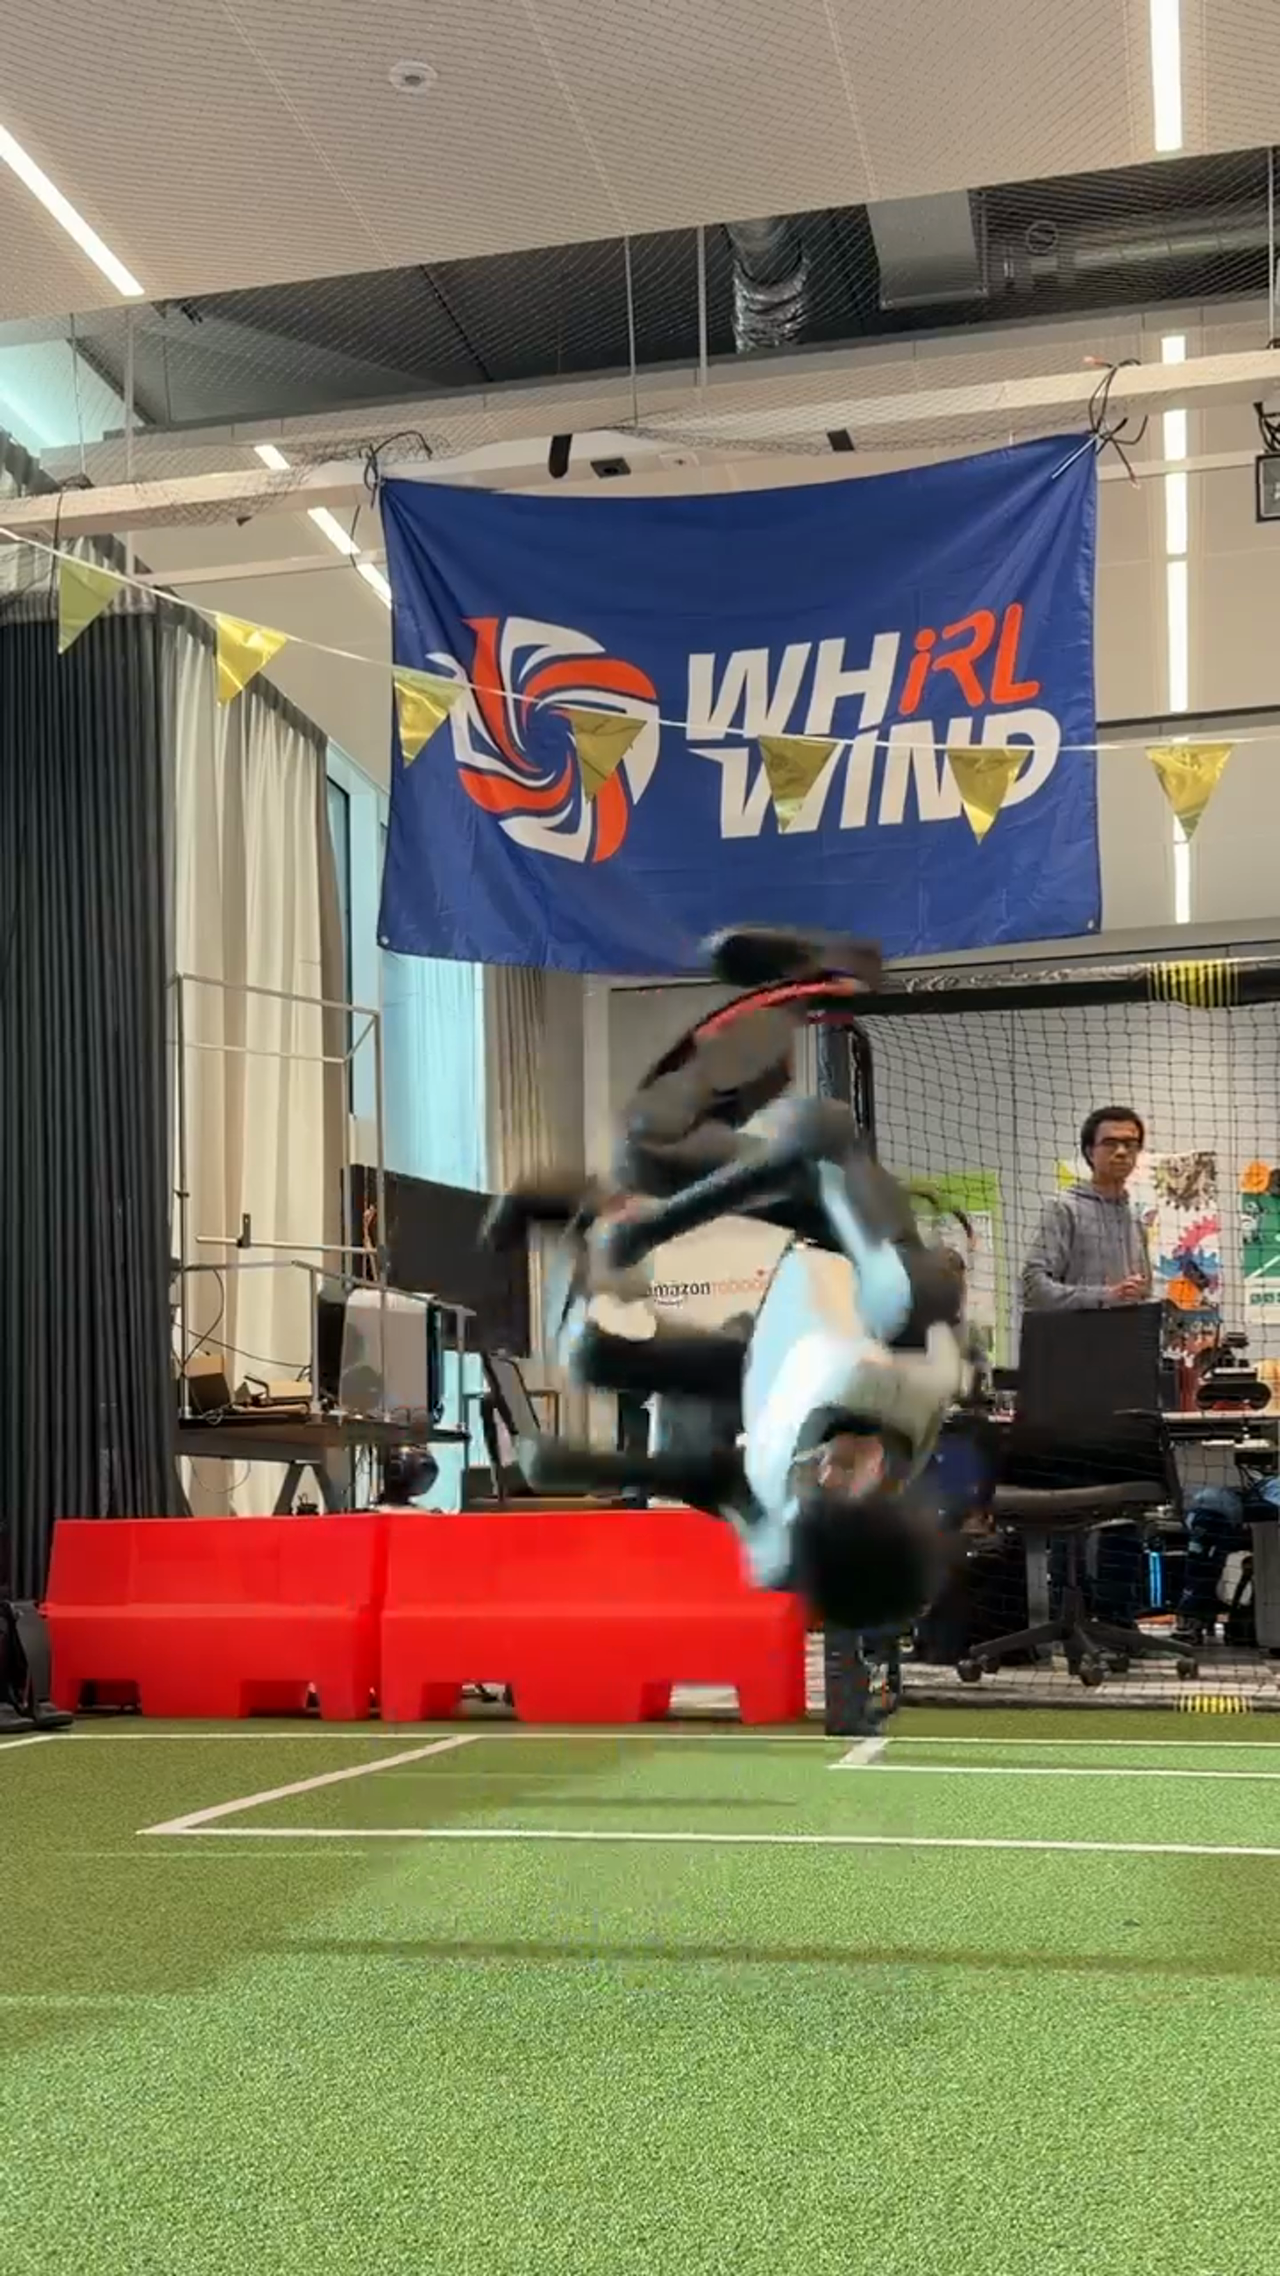
\includegraphics[width=\linewidth]{webster_flip/05.png}
	\end{subfigure}

	\vspace{0.5em} % vertical gap between rows

	\begin{subfigure}[b]{0.19\textwidth}
		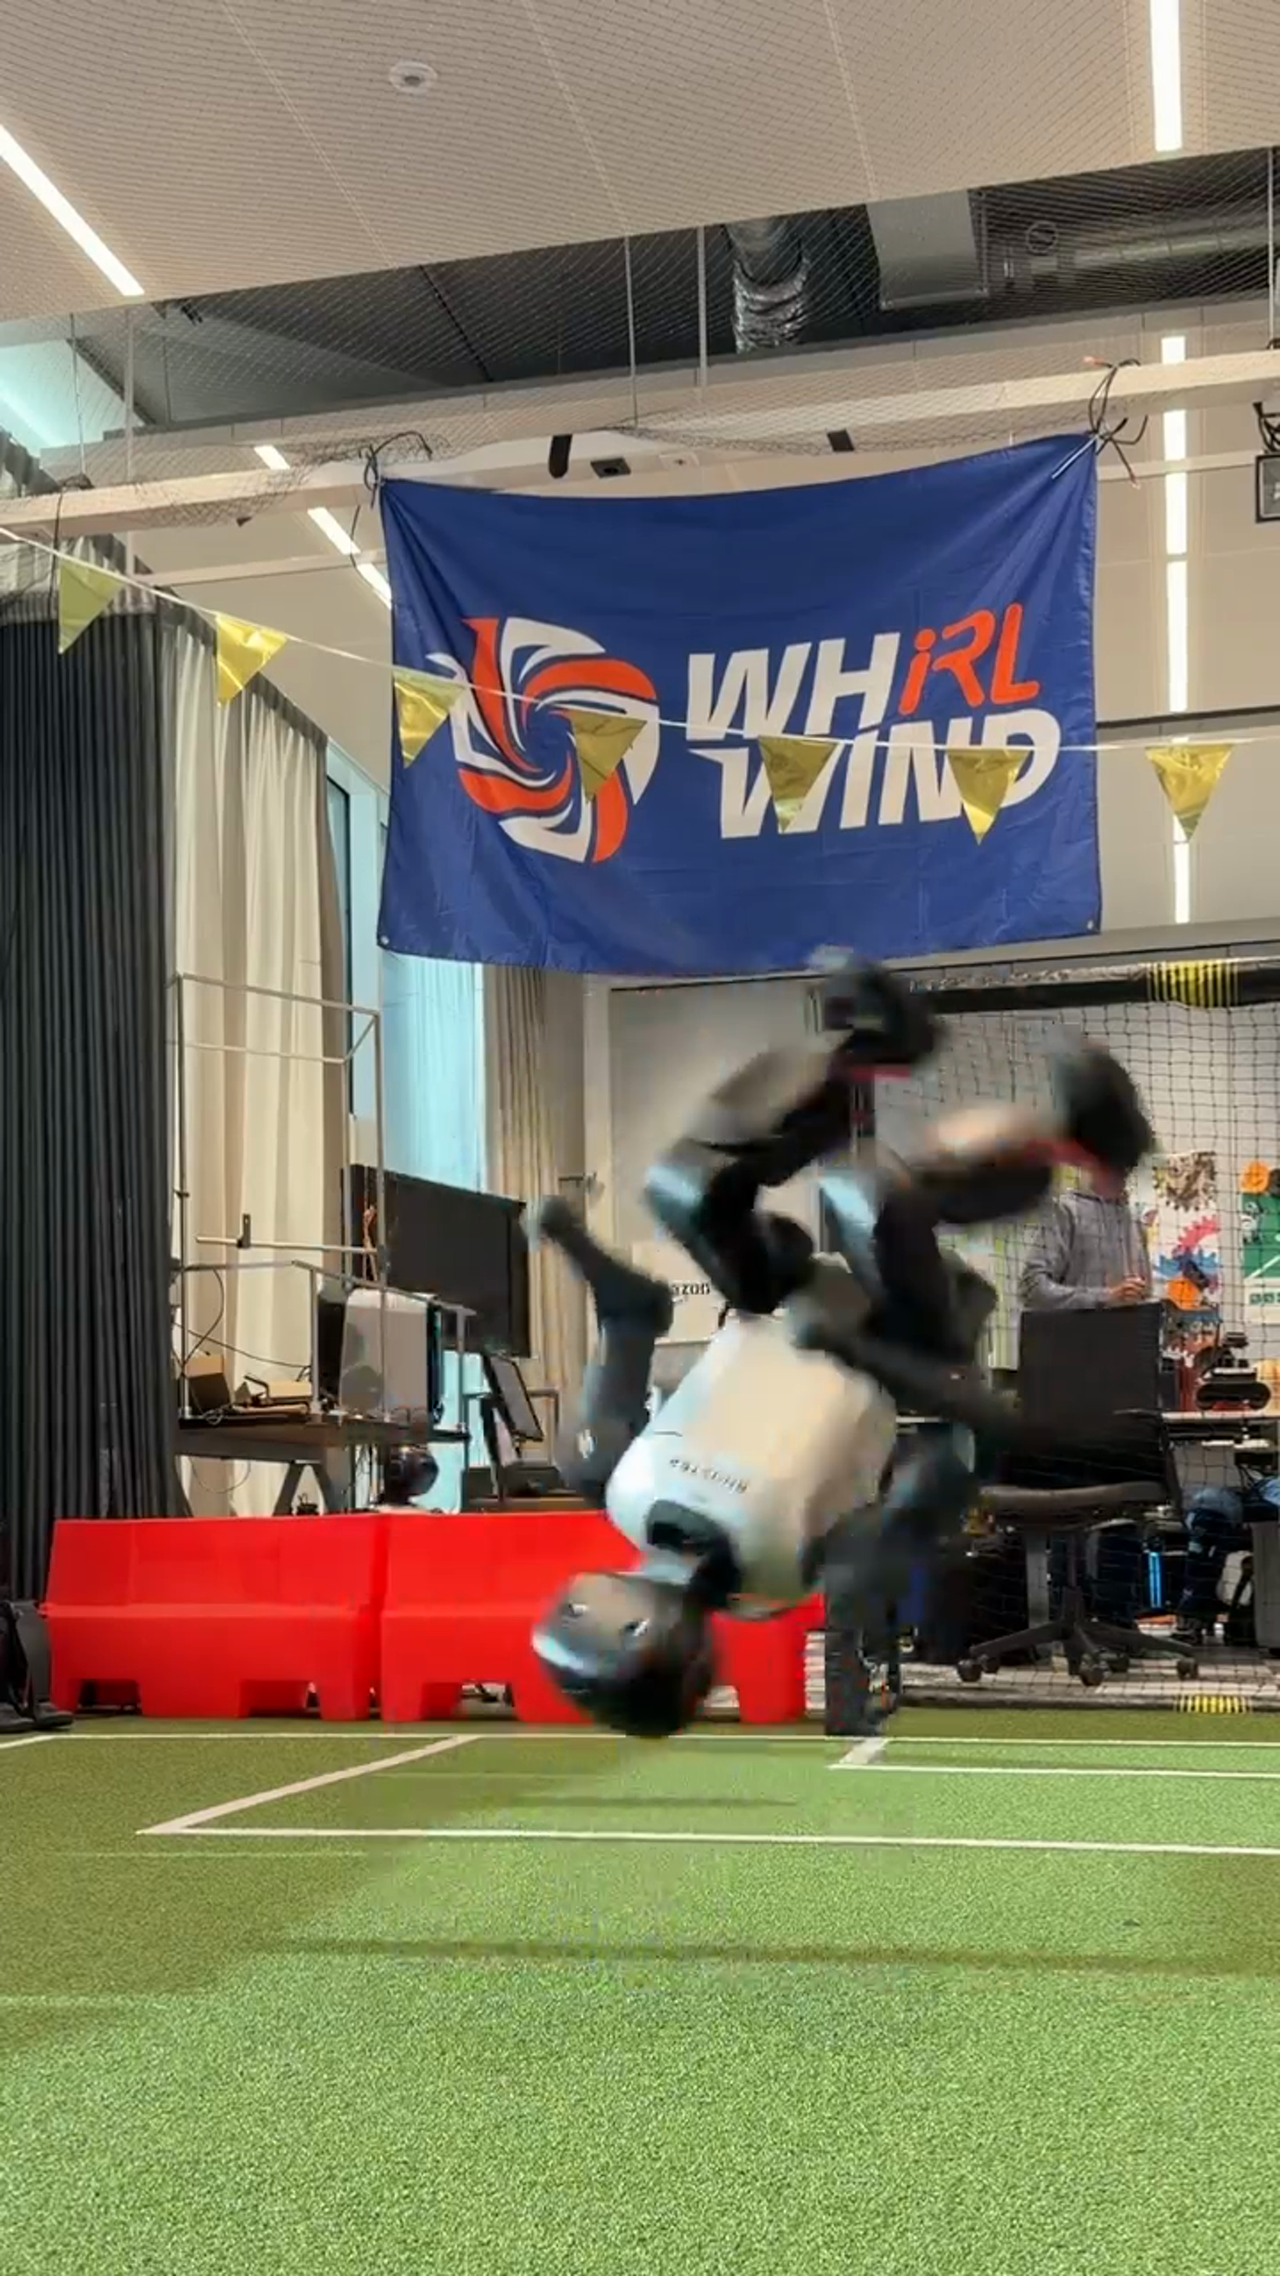
\includegraphics[width=\linewidth]{webster_flip/06.png}
	\end{subfigure}\hfill
	\begin{subfigure}[b]{0.19\textwidth}
		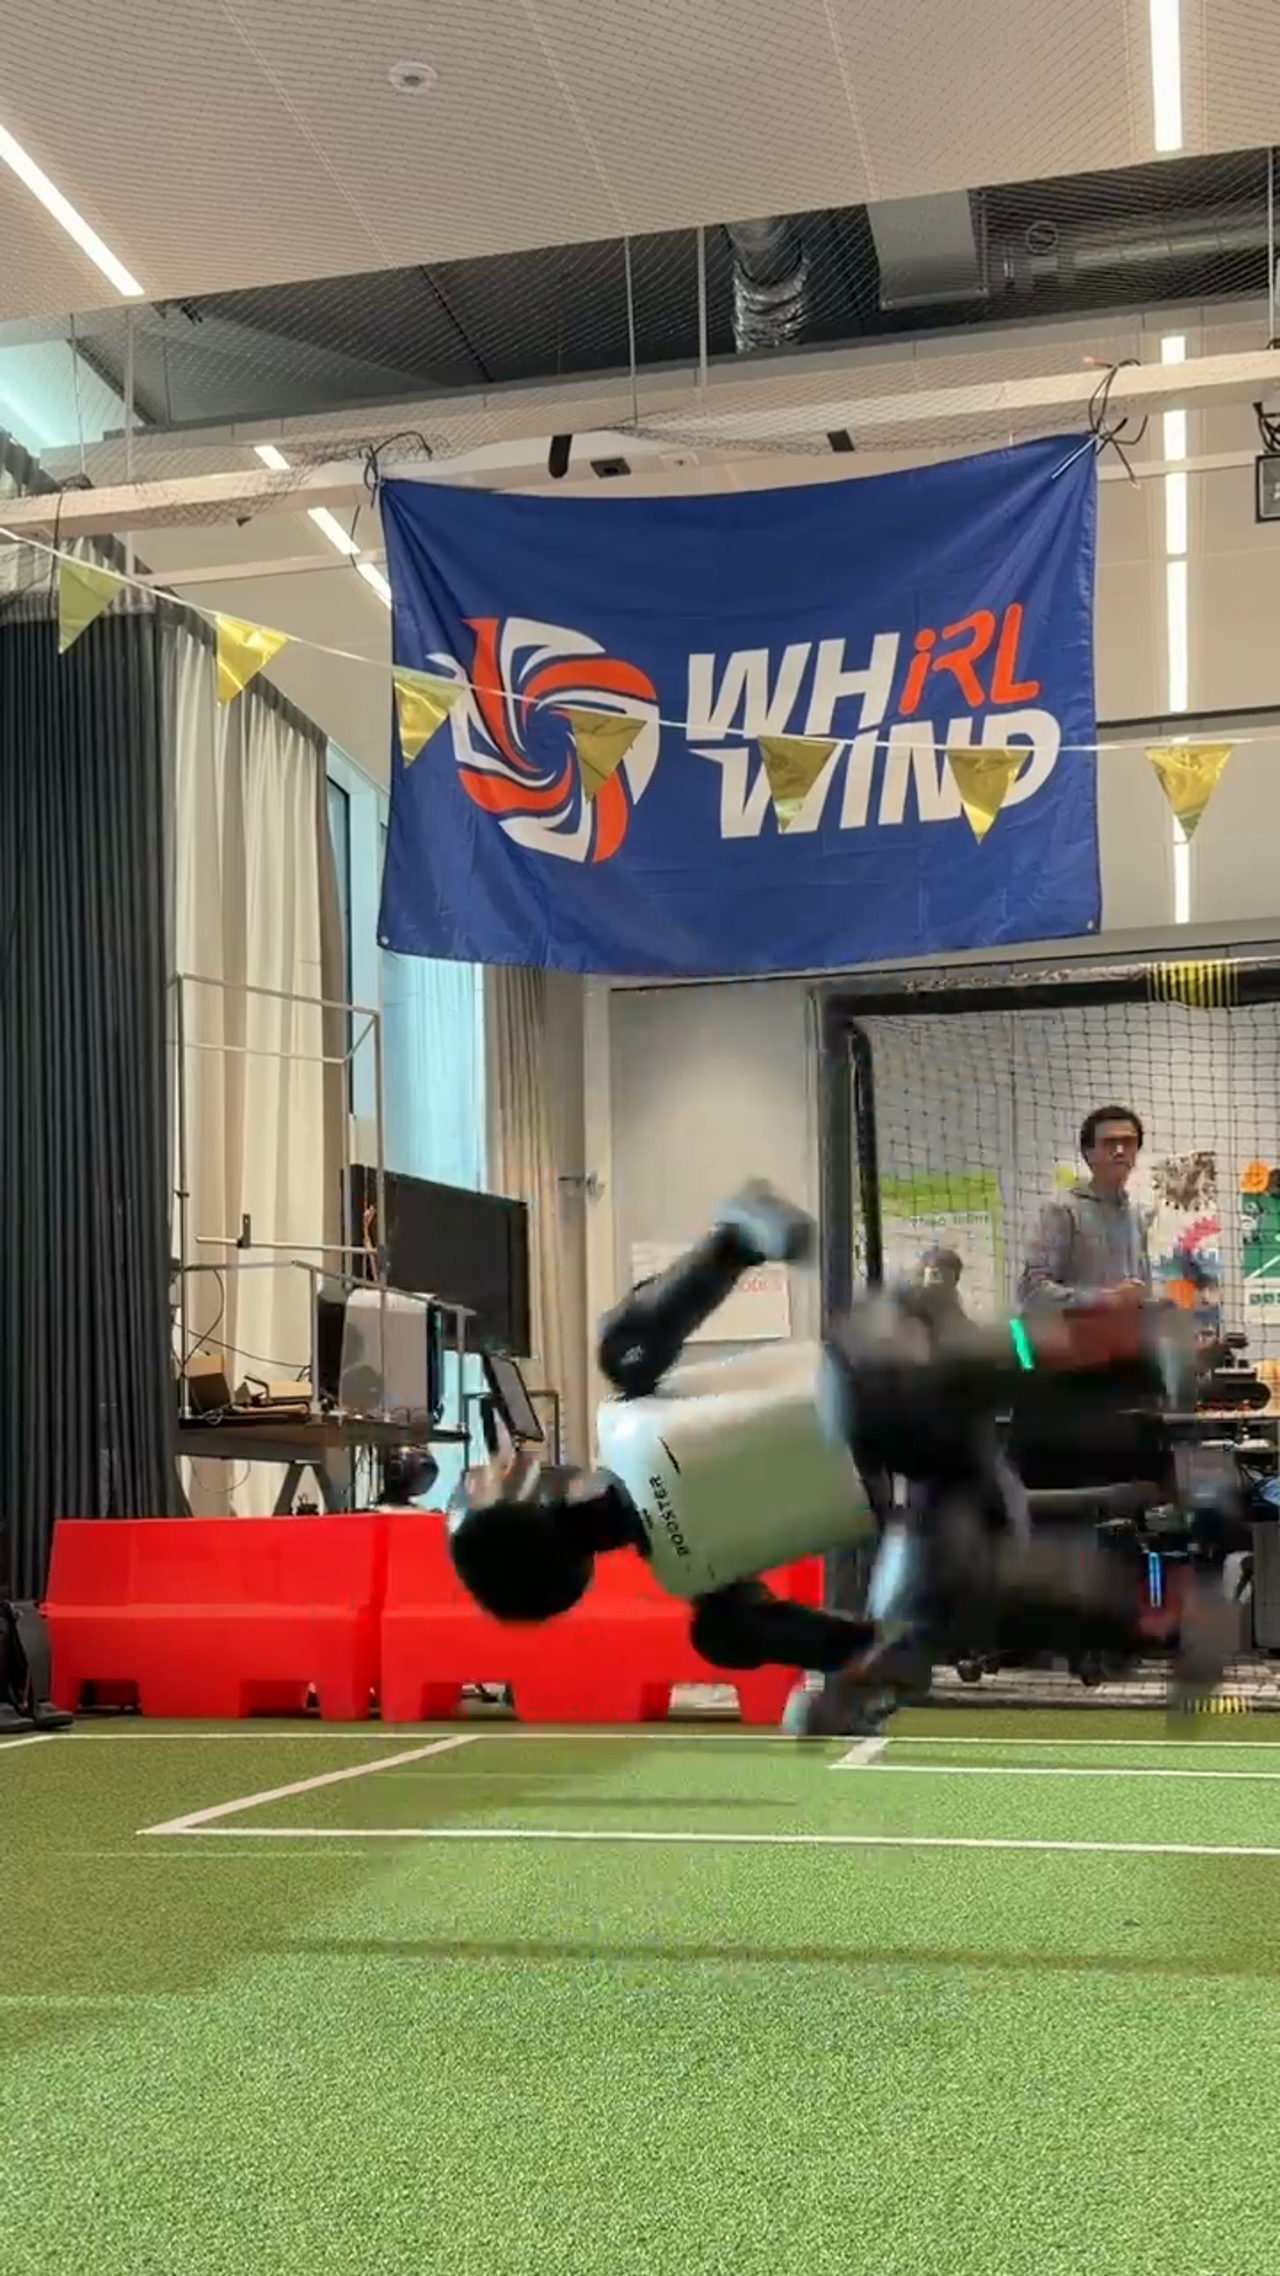
\includegraphics[width=\linewidth]{webster_flip/07.png}
	\end{subfigure}\hfill
	\begin{subfigure}[b]{0.19\textwidth}
		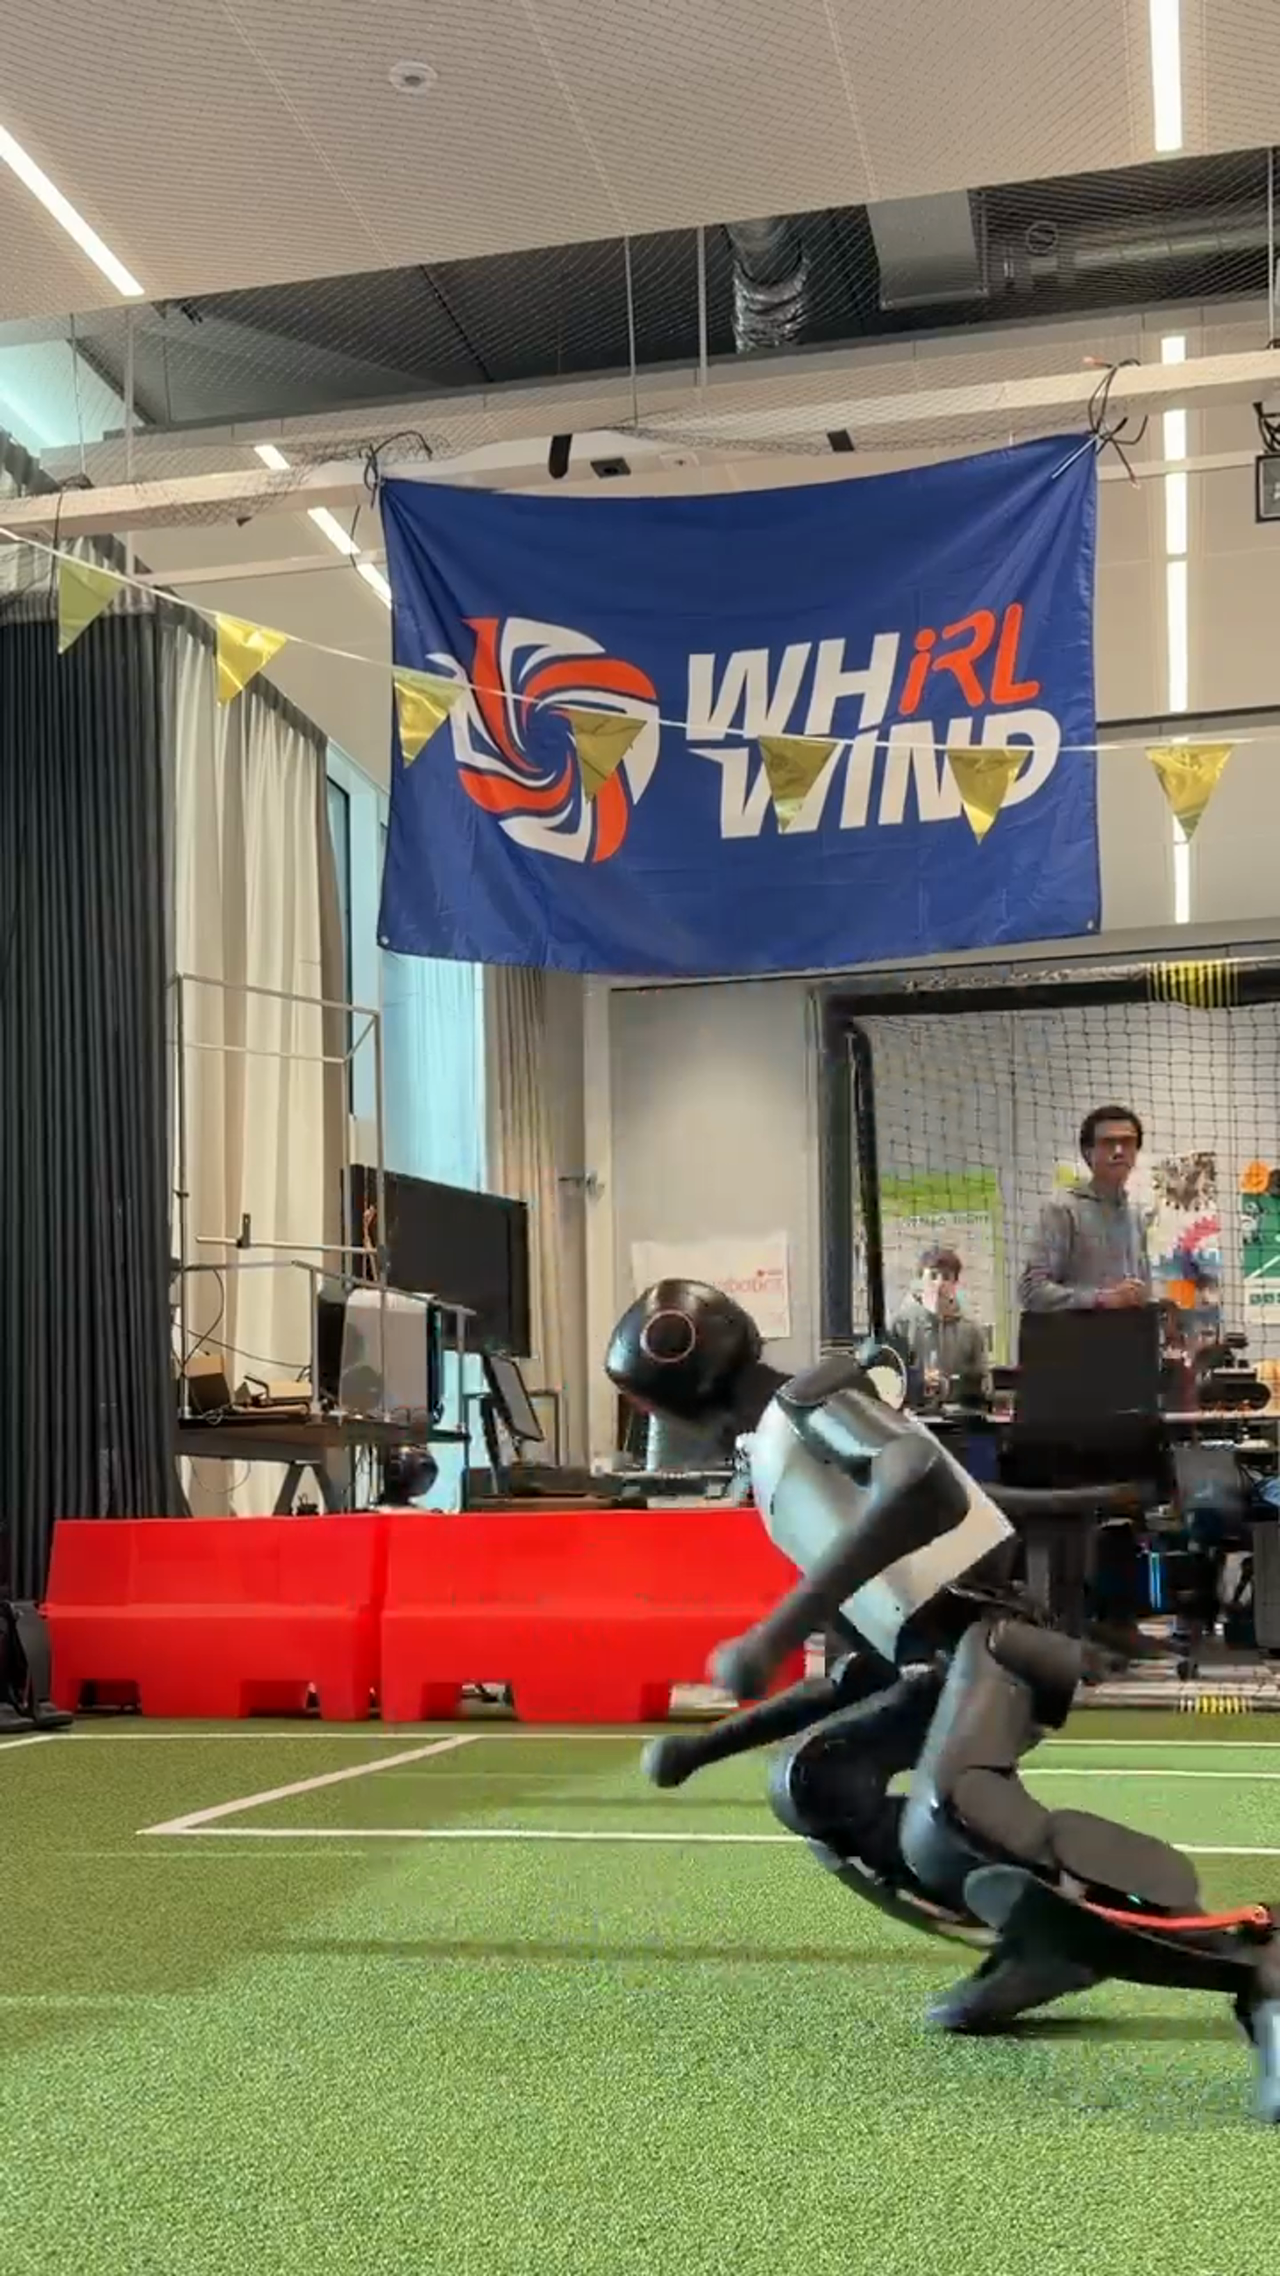
\includegraphics[width=\linewidth]{webster_flip/08.png}
	\end{subfigure}\hfill
	\begin{subfigure}[b]{0.19\textwidth}
		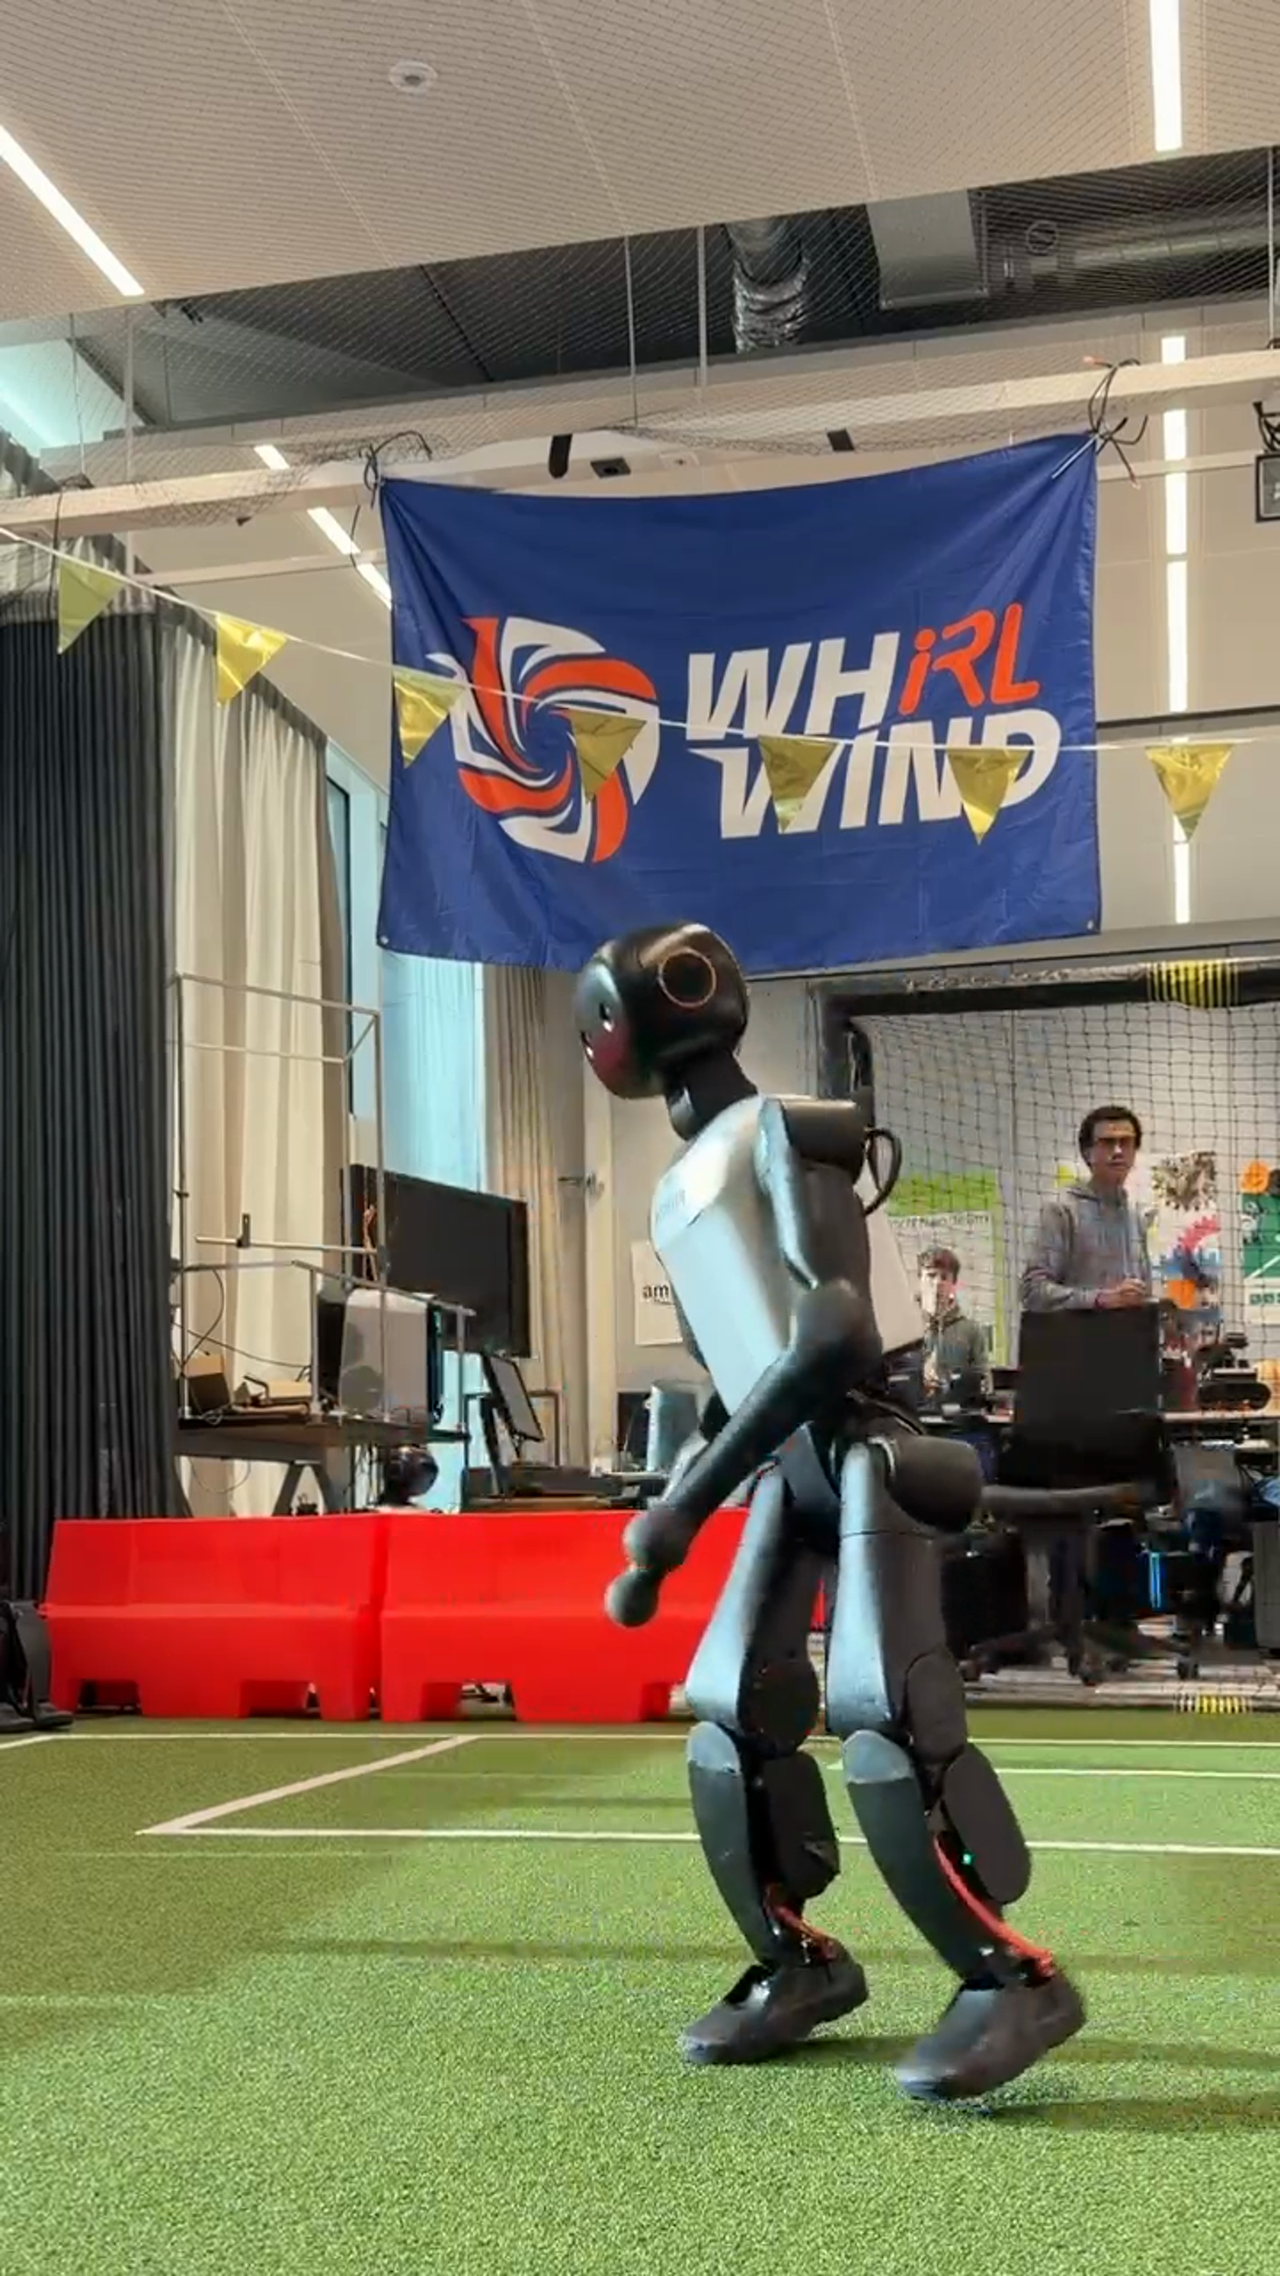
\includegraphics[width=\linewidth]{webster_flip/09.png}
	\end{subfigure}\hfill
	\begin{subfigure}[b]{0.19\textwidth}
		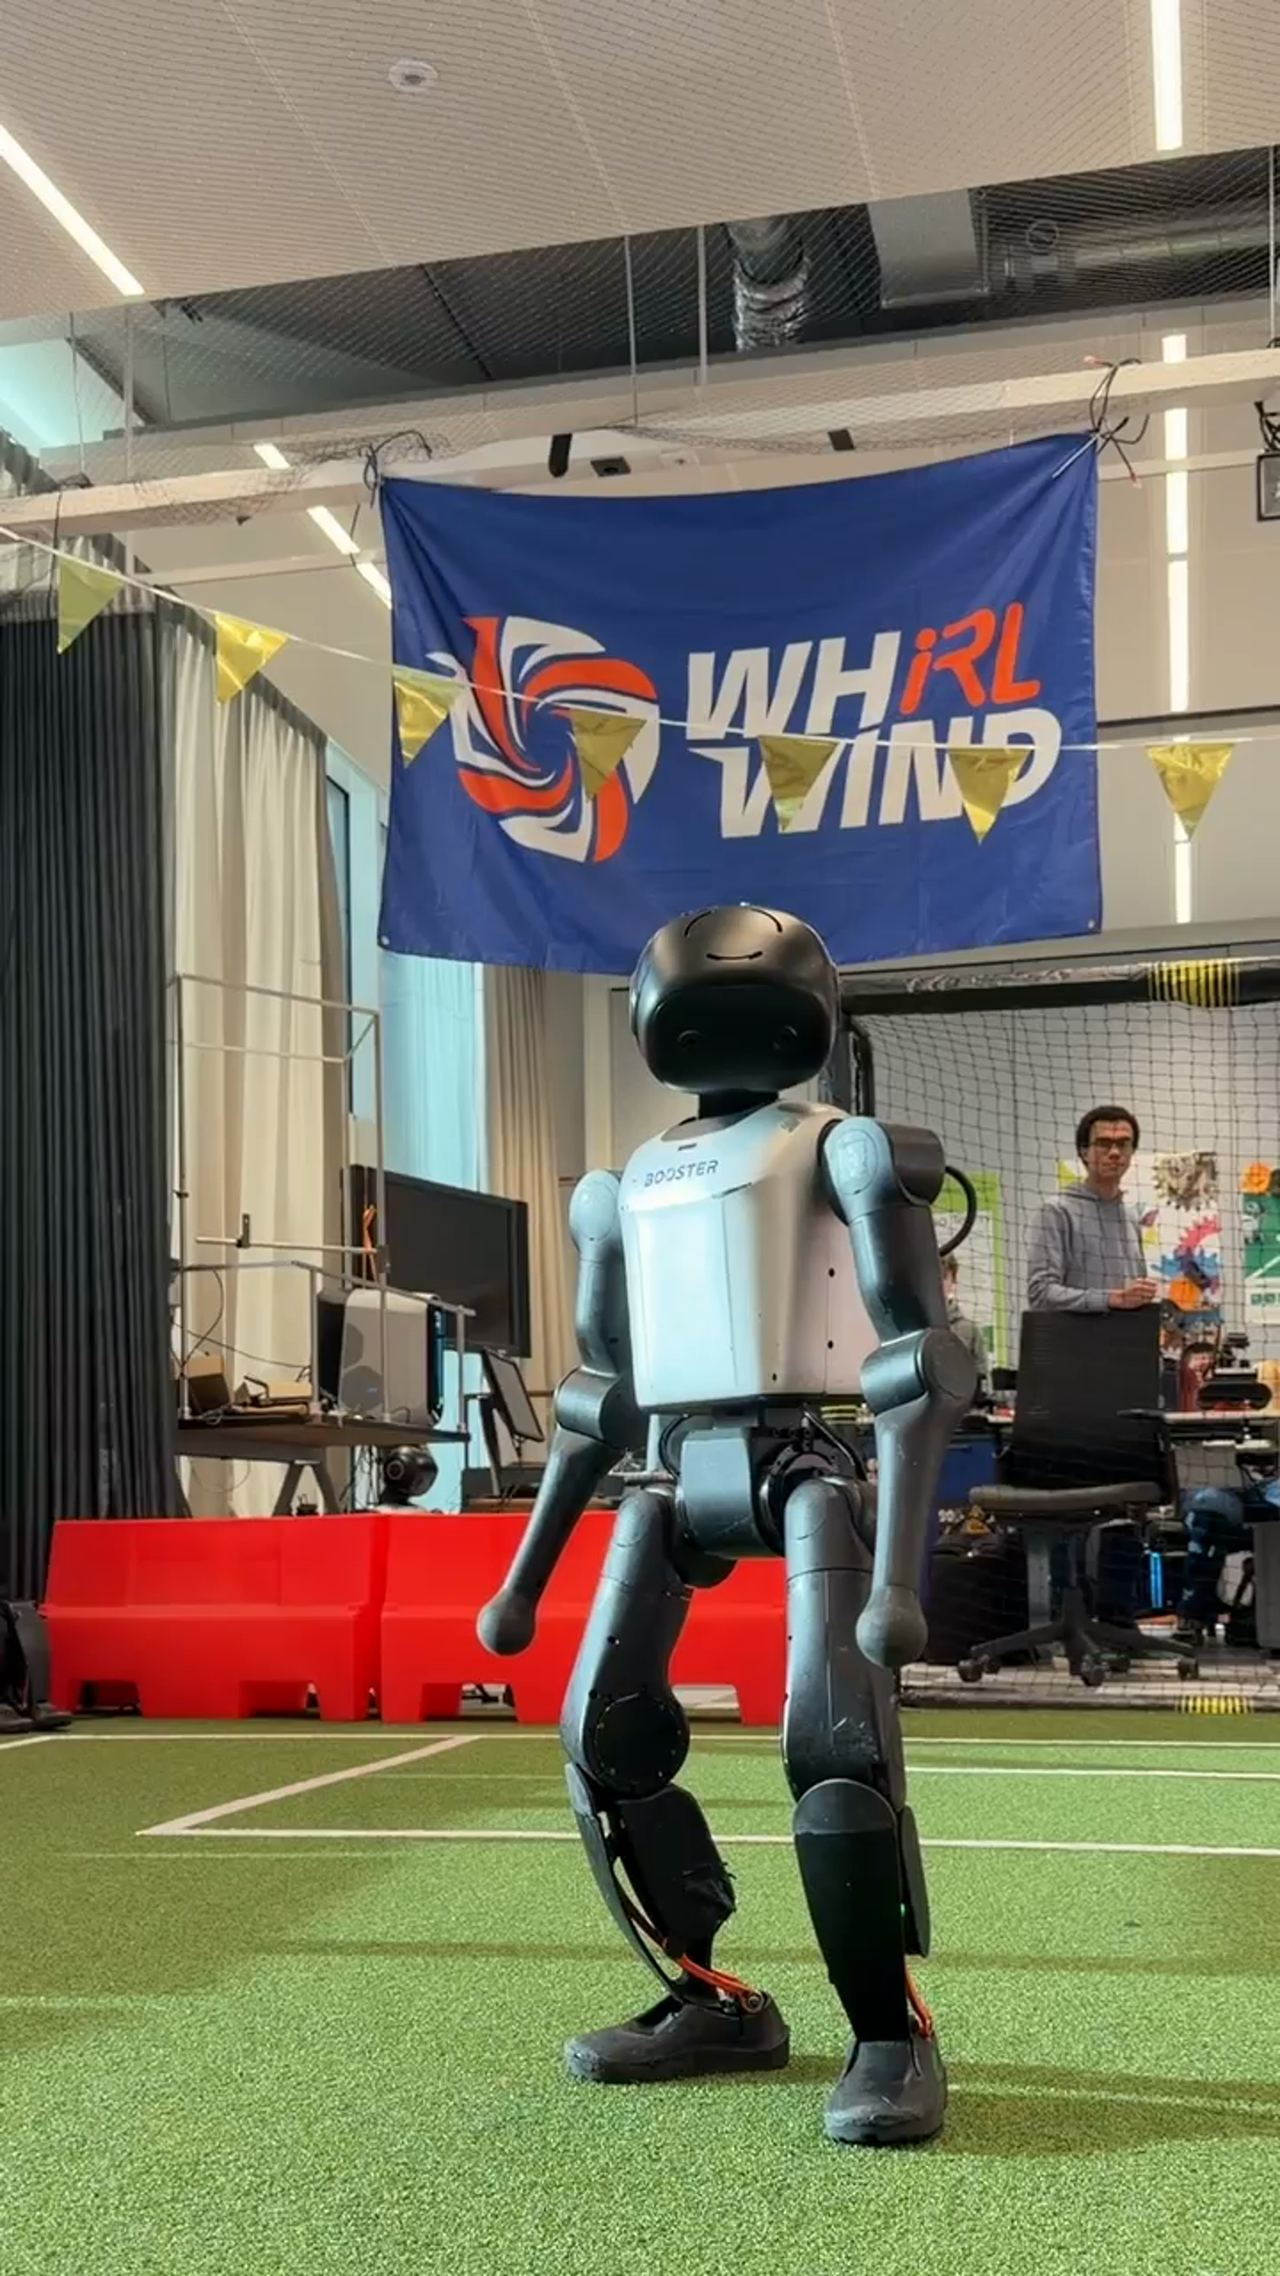
\includegraphics[width=\linewidth]{webster_flip/10.png}
	\end{subfigure}

	\caption{Booster K1 robot doing a webster flip}
	\label{fig:webster_flip}
\end{figure}

During such a motion the robot has to know at every moment how all its joints are bent (angles and trigonometry), where its feet, hands and head are (vectors and matrices), how fast everything rotates and how quickly that changes (derivatives), and how to correct small errors before it falls over (gradients and learning). A modern controller for a motion like this is often a \emph{neural network} that has been trained, and training is nothing but the calculus of this book at work.

\section*{Soccer as a grand challenge}
The flip is only one example of a complex motion. Soccer is full of them: a player has to receive a pass and control the ball, sprint and change direction in a split second, tackle an opponent without fouling, or, as a goalie, jump and catch a shot. All of these demand the same skills as the flip: balance, precise joint control and fast decisions. Soccer therefore combines many hard motion problems in one game, and this is why researchers let robots play it.

The RoboCup federation explains it on its website: RoboCup uses soccer as a long-term challenge to advance robotics and AI research, a ``landmark project'' and a ``standard problem'' on which many teams can compare their ideas\footnote{RoboCup Federation, \emph{Objective}, \url{https://robocup.org/objective}.}. The official long-term goal is:

\begin{quote}
\emph{By the middle of the 21st century, a team of fully autonomous humanoid robot soccer players shall win a soccer game, complying with the official rules of FIFA, against the winner of the most recent World Cup.}
\end{quote}

The organisers call this a grand challenge for the next decades that will not be met in the near future. On the way, the modest goal is to build a robot soccer team that plays like human players.

\section*{What makes it so hard?}
Compared with a game like chess, robot soccer is a much harder problem. The RoboCup objective page names several reasons\footnote{Source of the list and of the research areas below: the same RoboCup objective page.}, and each of them connects to a part of this book:

\begin{center}
\renewcommand{\arraystretch}{1.35}
\begin{tabular}{>{\raggedright\arraybackslash}p{4.3cm}>{\raggedright\arraybackslash}p{4.3cm}>{\raggedright\arraybackslash}p{4.2cm}}
\textbf{Challenge} & \textbf{What it means} & \textbf{Math you will learn}\\ \hline
Dynamic environment & The world keeps changing, unlike a chess board. & Functions, rates of change (Chapters~\ref{ch:functions}--\ref{ch:activation} and \ref{ch:rate}--\ref{ch:integrals})\\
Real-time play & There are no turns: decisions are needed now. & Fast computations with vectors and matrices (Chapters~\ref{ch:vectors}--\ref{ch:rotation})\\
Incomplete information & A robot sees only part of the field. & Coordinates and reference frames (Chapters~\ref{ch:coordinates}--\ref{ch:frames})\\
Raw sensor data & Cameras and sensors deliver numbers, not ``ball at $(4,5)$''. & Geometry, distances, vectors (Chapters~\ref{ch:coordinates}--\ref{ch:rotation})\\
Distributed control & Every robot decides for itself. & Neural networks (Chapter~\ref{ch:nn})\\
Motor control and learning & Walking, kicking and flipping need precise motions. & Trigonometry, matrices, gradient descent (Chapters~\ref{ch:coordinates}--\ref{ch:integrals})\\
\end{tabular}
\end{center}

The same page lists the research areas that RoboCup brings together: sensor fusion, reactive behaviour, multi-agent systems, real-time planning, learning and motor control. All of them are built on the topics you are about to study.

\begin{keyidea}[Your goal]
By the end of this book you will understand the mathematics behind a neural network that learns, and behind the geometry that tells a robot where it is and how to move. This is the foundation on which a robot, one day, can play like a champion.
\end{keyidea}
